\section{Discussion}
In the absence of ground truth, we used repeatability and prediction of
demographic variables to compare the ANTs and FreeSurfer cortical 
thickness pipelines.  One very important
issue that was not discussed in this work is quality control for
ensuring proper pipeline processing.  The time required to go through 
approximately 1,200 sets of results ($\times 2$ for both pipelines) would be
enormous (not to mention the tedium).  However, the first
author did do this for the brain extraction step to ensure that both pipelines
were achieving expected intermediate results.  The only
major failure was the FreeSurfer brain extraction of
a single IXI subject (IXI430-IOP-0990).
Also, three NKI subjects were not processed to completion
with FreeSurfer (1713515, 18755434, and 2674565) and were not included in the analysis.
Although  researchers might quibble over processing minutiae such as the
inclusion of too much (or not enough) of the meninges, we approached
our evaluation using more objective criteria which concern all those
engaged in this type of research.  We are currently trying to develop methods
to facilitate data inspection for quick quality assurance/control.

%\begin{figure}[htb]
%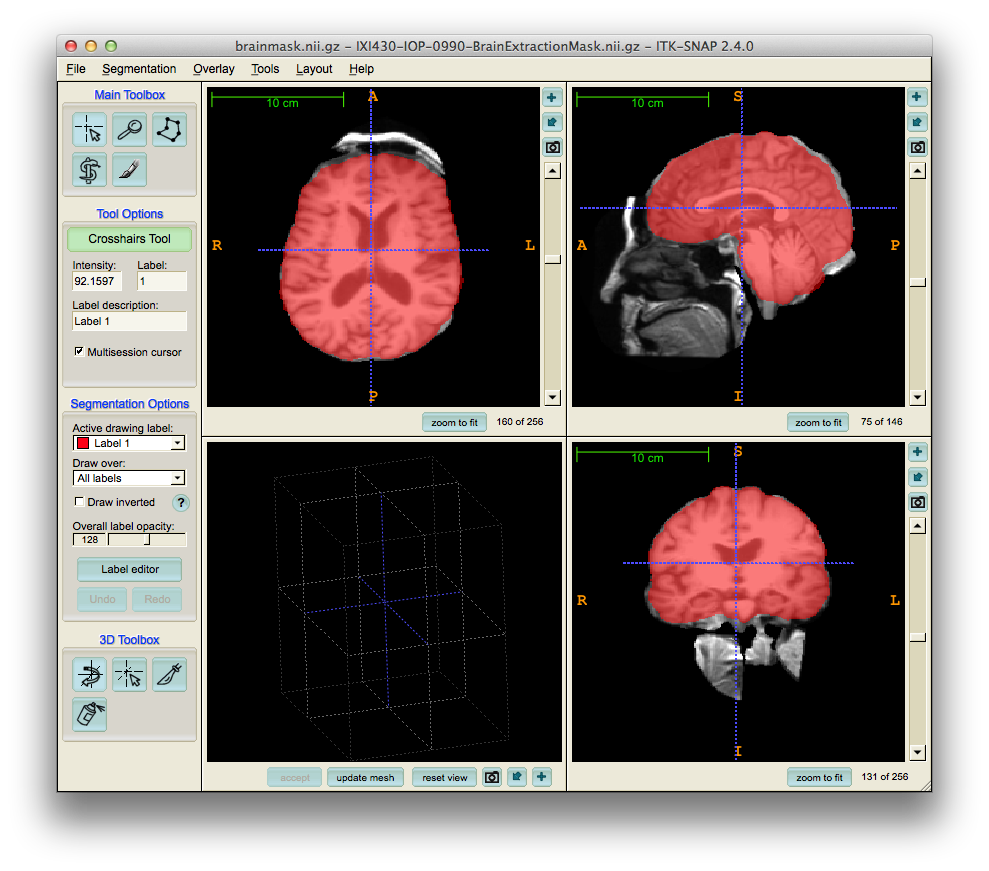
\includegraphics[width=87.5mm]{IXI430.png}
%\caption{A single FreeSurfer brain extraction failure for an IXI subject.  We 
%         overlay the ANTs-estimated brain mask for comparison.}
%\label{fig:ixi430}
%\end{figure}

\subsection{Repeatability of thickness measurements}
The OASIS data set 
and the MMRR data set allow us to test whether the same
thickness values emerge from T1-weighted
neuroimages collected on the same subject but at different times of
the day or over a time separation within a few weeks.  Given confounds 
such as short-term alterations due to T1-weighted susceptibility to
blood flow \cite{Franklin2013,Salgado-Pineda2006,Yamasue2007} and
longitudinal variation in scanner conditions, 
this strategy is not ideal.  However, related
tools have looked at this question. 
An independent evaluation of the FreeSurfer pipeline shows good
repeatability measurements \cite{jovicich2013}. The authors report
FreeSurfer reproducibility in the range of 1.5 - 5\% depending on the
//WHAT DO THESE \%s MEAN? AVG \% DIFFERENCE ACROSS ALL VERTICES FOR A GIVEN REGION?//
site and region of the brain.  A similar study found good
repeatability properties although the segmentation accuracy was worse 
than other popular segmentation methods \cite{eggert2012}.
//WOULDN'T IT BE IMPORTANT TO REPORT THESE RESULTS?//
The CLADA pipeline showed the ability to detect
changes as small as 1 millimeter and showed good agreement with
FreeSurfer \cite{nakamura2011}.
//HOW GOOD?  WHAT WAS THE MEASURE OF GOODNESS?  WHY NOT USE CLADA?//

Very recently, it was suggested that 3T MRI
consistently overestimates cortical thickness \cite{lusebrink2013}.
Repeatability of thickness estimates in that study were in the range
of 0.2 mm //WHAT THICKNESS MEASURE/SOFTWARE?
AVG'D ACROSS ALL VOXELS/VERTICES PER REGION?//
although the study design differs substantially from that used here.
In summary, our results (though computed
with a different cortical parcellation) are competitive.  //HOW COMPETITIVE, AND WITH WHAT?//
Finally, some users may choose to segment and register
with ANTs and subsequently employ any alternative (e.g.,surface-based)
method for thickness estimation.  Further work is needed by
independent authors working on established pipelines (as in \cite{lusebrink2013,jovicich2013})
to better compare surface-based and volume-based thickness reliability
across different populations and age ranges. 

\subsection{Age and gender prediction} 
Although repeatability between ANTs and FreeSurfer is comparable,
such measures are not as useful in determining the utility of the 
measuring software.  That is the reason we use //PAST TENSE IS USED BELOW//
a training and testing paradigm to evaluate how well both frameworks produce measurements
capable of predicting demographics which are well-known to correlate
with cortical thickness.  Additionally, these demographic measures are
probably some of the easiest and most reliably obtained of all possible
demographic measures used for this type of assessment.  For age prediction,
we used both a linear model (due to its general ubiquity) and a random
forest model (a non-parametric model to contrast with the linear approach)
which showed overall good performance.  Also, the linear  and
random forest models have the advantage of being
interpretable.  That is, the models reveal the specific predictors
that are most valuable which will be explored in future work.  

\subsection{Computation time}
Computation time for the registration and segmentation components of
the ANTs pipeline are substantial.  It is likely that nearly as reliable
results can be obtained in much less time for many of the subjects in
this study.  However, our interest in
maximizing reliability and quality led us to employ parameters in the
registration, segmentation, and bias correction that are as robust as
possible to differences in head position, the presence of large
deformations between template and target brains and substantial
inhomogeneity or other artifacts in the image content itself.  Several
subjects (e.g., NKI: 1898228, 1875434) provide examples of more difficult
data from which we are able to
extract meaningful segmentations and registrations, despite the presence of a
``garbage-in/garbage-out'' problem.  A subject of future study is
determining an exact cut-off for the inclusion of such data.  We do not
investigate this issue here, which has concerned statisticians for over
half a century \cite{Hampel2001}. 

\section{Conclusions}

Imaging biomarkers such as cortical thickness play an 
important role in neuroscience research.  Extremely useful to
researchers are robust software tools for generating such 
biomarkers.  In this work we detailed our open source offering for estimating
cortical thickness directly from T1 images and demonstrated
its utility on a large collection of public brain data from
multiple databases acquired at multiple sites.  To our knowledge,
this study constitutes the largest collection of cortical
thickness data processed in a single study.  
We anticipate that public availability of our tools and extensive tuning on
the specified cohorts will prove useful to the larger
research community.   In this work, we only explored a portion of the potentially
interesting investigations possible with these data.
Since all of the data are publicly available, further work can
be easily pursued by us or by other interested groups.